\section{EXPERIMENTAL SETTING AND RESULTS}
\label{sec:mot}

\begin{table}
\centering
\caption{Benchmark information}
	\begin{tabular}{l}
	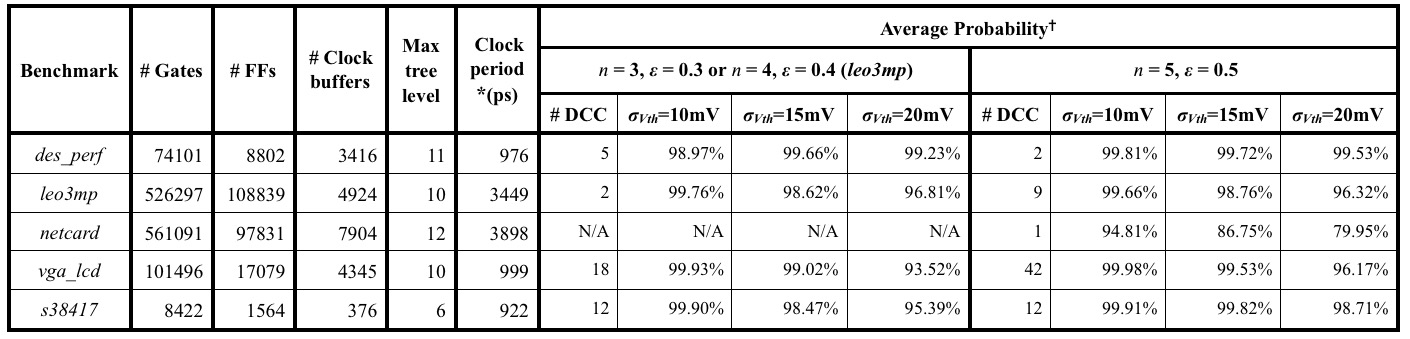
\includegraphics[width=0.85\columnwidth]{./experiment/benchmarkinfo.png}
	\end{tabular}
\label{table:benchmark}
\end{table}

%%---------TEST--------------
\begin{figure*}[!ht]
    \centering
    \subfigure[\textit{s38417} is attacked with $n$ = 3 yr and $\varepsilon = 0.3$ yr]{
    	\label{fig:sub:s38417_3y}
        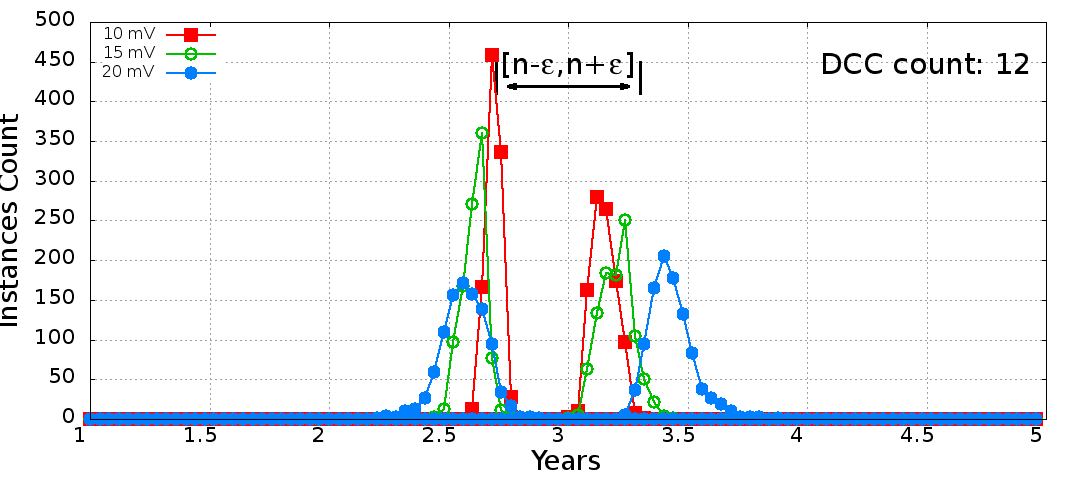
\includegraphics[width=0.8\columnwidth]{./experiment/s384173y.png}
    }
    \hspace{0.1cm}
    \subfigure[\textit{s38417} is attacked with $n$ = 5 yr and $\varepsilon = 0.5$ yr]{
    	\label{fig:sub:s38417_5y}
        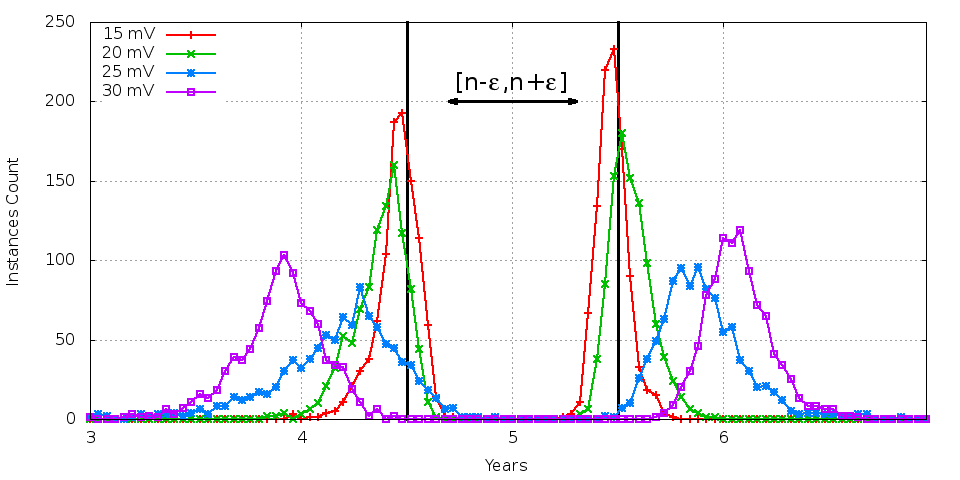
\includegraphics[width=0.8\columnwidth]{./experiment/s384175y.png}
    }
    \hspace{0.1cm}
    \subfigure[\textit{des\_perf} is attacked with $n$ = 3 yr and $\varepsilon = 0.3$ yr]{
    	\label{fig:sub:des_3y}
        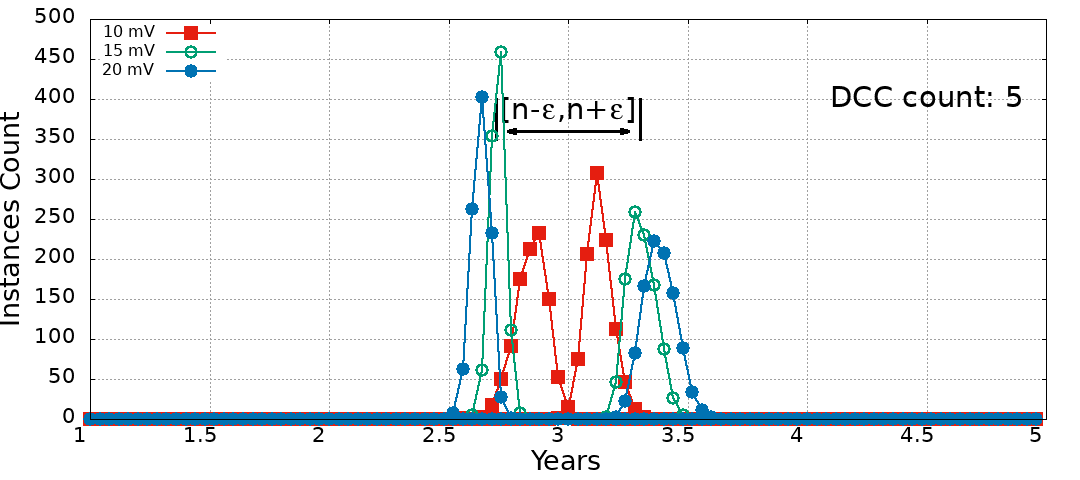
\includegraphics[width=0.8\columnwidth]{./experiment/des3y.png}
    }
    \subfigure[\textit{des\_perf} is attacked with $n$ = 5 yr and $\varepsilon = 0.5$ yr]{
    	\label{fig:sub:des_5y}
        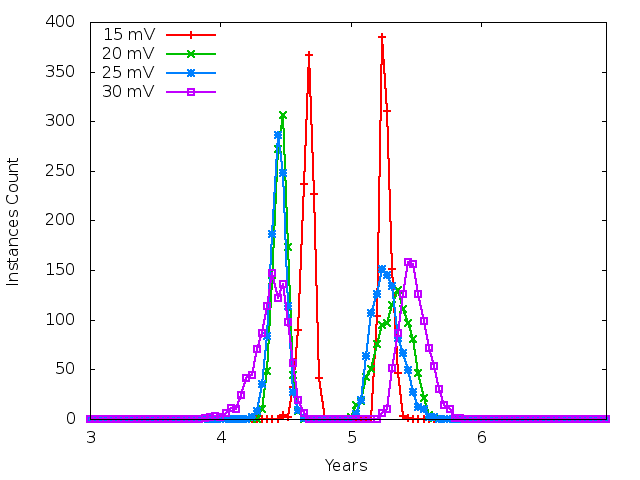
\includegraphics[width=0.8\columnwidth]{./experiment/des5y.png}
    }
    \subfigure[\textit{leo3mp} is attacked with $n$ = 4 yr and $\varepsilon = 0.4$ yr]{
    	\label{fig:sub:3mp_3y}
        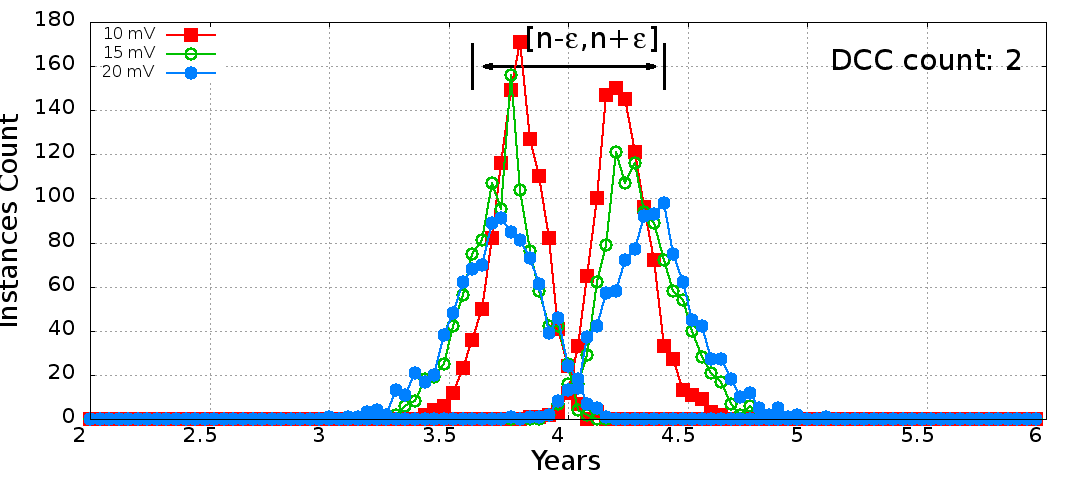
\includegraphics[width=0.8\columnwidth]{./experiment/3mp4y.png}
    }
    \hspace{0.1cm}
    \subfigure[\textit{leo3mp} is attacked with $n$ = 5 yrs and $\varepsilon = 0.5$ yr]{
    	\label{fig:sub:3mp_5y}
        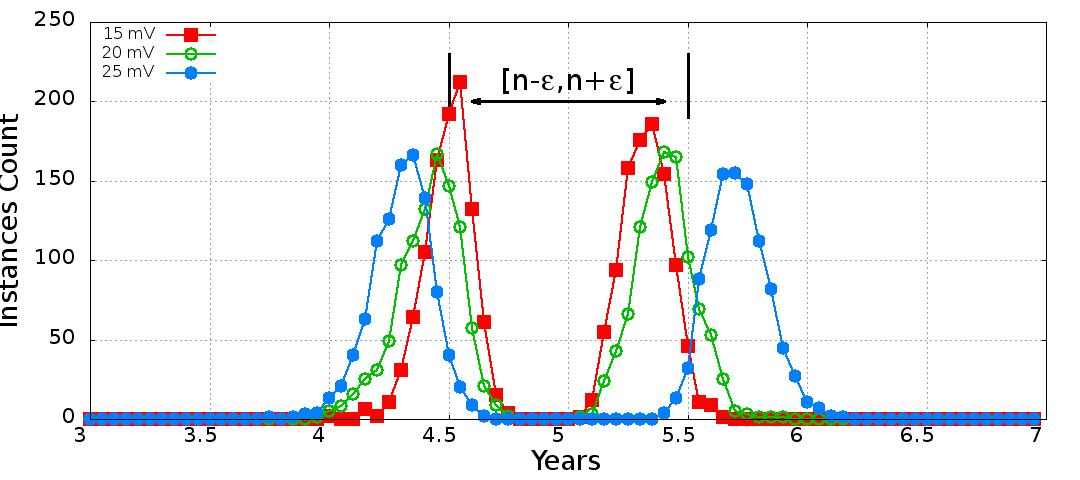
\includegraphics[width=0.8\columnwidth]{./experiment/3mp5y.png}
    }
    \caption{Lifetime distributions of Monte-Carlo Instances of Trojan-included \textit{s38417}, \textit{des\_perf}, and \textit{leo3mp}}
    \label{fig:exp}
\end{figure*}

\subsection{Experimental Setting}
\label{sec:exp:tc}
In our experiments, the benchmarks are picked out from IWLS'05 and ISCAS'89. The utilized technology is TSMC 65nm GP standard cell series. The utilized SAT solver is MiniSAT 2.2. The information of each design/benchmark is reported in Table~\ref{table:benchmark}, where the clock periods (Column 6) are specifically set to make the designs fail at the specified time (in our experiment, 7 years) in the presence of aging. The resulting clock period is both used in Trojan-free and Trojan-included (attacked) designs. 
\subsection{Monte-Carlo Instantiation of the Attacked Designs}
\label{sec:ins:mc_ins}
Given an attacked design, each Monte-Carlo instance of the design is generated by imposing extra $V_{th}$ offset (i.e., $\Delta V_{th}$ ) on each transistor. The $V_{th}$ offsets follow a normal distribution with the standard deviation ($\sigma_{V_{th}}$) of a given value (usually 10mV$\sim$25mV~\cite{han2011statistical}\cite{schlunder2017influence}). Each instance (i.e., Monte-Carlo seed) can be viewed as a die. In our experiment, each attacked design is instantiated for 1000 times with a specified value of $\sigma_{V_{th}}$. 
%\subsection{Lifetime Estimation Considering the Effect of PVs on Aging Rates of Transistoras}
%\label{sec:ins:lt}
Then, we estimate the lifetime interval of each instance based on the method proposed in Section~\ref{sec:lt_estimation}. Note that, because threshold voltages of transistors are not the same due to PVs, their aging rates differ with each others. As a consequence, we cannot use the deterministic Equation (\ref{eq:worst}) to derive the severe aging rates of candidate paths. Instead, we derive the aging rate of individual transistor based on the mathematical model in Section~\ref{sec:frame} regarding the correlation between PVs and BTI.

\subsection{Lifetime Distribution of Monte-Carlo Instances}
\label{sec:exp:exp}
Figure~\ref{fig:exp} shows the lifetime distributions of instances of the attacked three designs (\textit{s38417}, \textit{des\_perf} and \textit{leo3mp}). The designs are attacked to fail at $3^{rd}$, $4^{th}$\footnote{Note that, there exists no SAT solution while \textit{leo3mp} is attacked to fail at $3^{rd}$ year, whereas there exists SAT solution while it is attacked to fail at $4^{th}$ year.} or $5^{th}$ year (i.e., $n = 3, 4, or 5$). In each subfigure, there exist three distributions, each of distributions corresponds to one standard deviation of $V_{th}$ ($\sigma_{V_{th}}$) while generating Monte-Carlo instances. In our experiments, the $\sigma_{V_{th}}$ is set to 15mV, 20mV, and 25mV, respectively. As we can observe in each distribution, there exist two peaks. The left/right peak denotes the distribution of lower/upper bounds of lifetime intervals of instances. Note that, the instances in Figure~\ref{fig:exp} are instantiated from Trojan-included designs, instead of Trojan-free counterparts, whose lifetimes are not subject to PVs. Thus, we do not generate the Monte-Carlo instances for Trojan-free designs .

As shown in Figure~\ref{fig:exp} apparently, as $\sigma_{V_{th}}$ becomes larger, the interval between the left and right peaks becomes wider, indicating the larger $\sigma_{V_{th}}$ leads to fewer accurate attacks. Therefore, the lifetime accuracy of the proposed Trojan is impacted by the diversity of threshold voltages of transistors. Even though the peaks of two bounds deviate from the desired lifetime interval $[n - \varepsilon, n + \varepsilon]$, it does not mean that the attacked designs must not fail in that interval. For the estimated lifetime interval of each instance, the lower/upper bound denotes the earliest/last time point that the instance will fail. The exact time points, at which the instances fail, depends on the workload. Since the lifetime interval of each instance is overlapped with the desired lifetime interval $[n - \varepsilon, n + \varepsilon]$, the proposed Trojan is still likely to control the design lifetime in that interval.

\subsection{Detectability of the Proposed Trojan Attack}
\label{sec:exp:det}
A side-channel analysis is a countermeasure often taken for detecting the existence of hardware Trojan. Nevertheless, the used DCC count is marginal compared with the total gate count. On average, DCC count is less than 0.2\% of total gate count. That is, the area overhead is insignificant. In addition, the power overhead due to DCCs can be regarded as the power variations caused by PVs. As a result, the proposed Trojan is difficult to detect by the conventional side-channel analysis. 

Some Trojan defenders can insert on-chip monitors in the clock network to inspect the variation of clock duty cycle. However, the method need extra I/O pins/ports, which is impractical because the pin counts of ICs are limited and the area overhead.


\section{CONCLUSION}
We proposed a framework of hardware Trojan insertion to control the circuit lifetime, considering process variations and aging correlations between pairs of critical paths. The influence of Trojan heavily reduce the lifetime of circuit instances. Even though the accuracy is impacted by PVs, the lifetime of instances is still likely to fail within the desired lifetime interval $[n - \varepsilon, n + \varepsilon]$. More important, the area overhead of inserted DCCs is less than an average of 0.2\% of total gate count, which implies the proposed Trojan is very difficult to detect and succeed in decreasing the lifetime of attacked designs.
